\documentclass{llncs}
\usepackage{makeidx}
\usepackage{graphicx}
\usepackage{subfigure}
\usepackage[portuges]{babel}
\usepackage[utf8]{inputenc}

\begin{document}
\title{RoboIME : Team Description Paper for RoboCup 2014}
\author{
 Andre O. P. Barcelos \and
 Douglas K. Paixão \and
 Jan L. L. Segre \and
 Lucas O. de Lima \and
 Naum A. F. Barreira \and
 Paulo F. F. Rosa \and
 Rafael C. Felzenszwalb \and
 Renan Gemignani \and
 Robinson C. M. B. Filho \and
 Vitor H. F. Betio \and
 Victor Bramigk
}

\institute{Instituto Militar de Engenharia (IME) \\ Praça General Tibúrcio, 80 - Praia Vermelha, Urca \\ Rio de Janeiro - RJ - Brazil \\ \email{roboime@googlegroups.com}}
\maketitle
%
\begin{abstract}
This paper describes the electronic, mechanical and software designs developed by RoboIME
Team in order to join RoboCup 2014. All designs are in agreement with the rules of Small
Size League 2014. This is the second RoboIME participation in a world level RoboCup event,
although the team was already challenged third in Brazilian competitions.
\end{abstract}

\section{Introduction}
    RoboIME is a small-size league soccer robot team from IME, Rio de Janeiro, Brazil. This
is only the third time the team is taking part in competitions. The main result was in 2012
when the team achieved second place in Latin American Robotics Competition.

All students that work in this project are members of the Laboratório de Robótica e
Inteligência Computacional at IME. The previous studies \cite{alexandre}\cite{marco} provided
the basis for the current structure of software and hardware team's. This paper describe the
computer, electronic and mechanical design.

\section{Software System}
	The software system consists basically of five modules: AI, LogPlayer, Simulated World,
Support Simulation and Transmission. The modules were implemented using the Microsoft Visual
Studio 2010 IDE, that allows a single solution integrated of projects in different programming
languages (e.g. CSharp, C++), making the project more flexible for other programmers giving
continuity to the implementation.

	We chose to adopt the fragmentation of the software project into modules to facilitating
the implementation team. A UDP socket interface was adopted for communication between most modules
giving independence to them. Some interfaces like between AI Module and Support Simulation Module,
that need high performance, don't communicate using the UDP Socket interface. Figure \ref{fluxogramaSoftware}
shows the block diagram of the software system.

\begin{figure}[thpb]
     \centering
     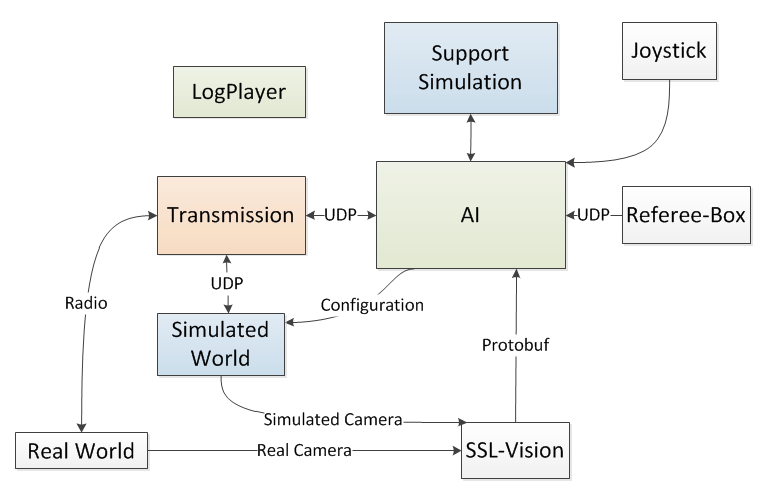
\includegraphics[scale=0.55]{img/fluxogramaSoftware.png}
     \caption{Block diagram of the software system}
     \label{fluxogramaSoftware}
\end{figure}

\subsection{AI Module}
	This is the largest and most complex software module. It is responsible for the following features:
\begin{itemize}
\item Collect, interpret and filter data from the Referee-Box, SSL-Vision, Transmission Module (real world or simulated), Support Simulation Module and Joystick;
\item Take high level decisions to define the actions that robot should do (i.e., to find the position
and orientation that robot has to reached, find the force to kick the ball, find the torque to dribble the ball);
\item Use the Support Simulation Module to create a planning;
\item Make a short future preview of the world (real or simulated) using data from the sensors (encoder, camera, infra-red);
\item Make the configuration of the simulation environment Simulated World (setting bodies existing in the simulation);
\item Control position and orientation of the robot defining which speeds the robot actuators (motor,
kicker and dribbler) must reach. These speeds will be passed to Transmission Module to be sent to the World (simulated or real);
\end{itemize}

	Among the many reactive behavioural control architectures, we have chosen STP (Skills, Tactics and Plays)
architecture \cite{STP}. In order to create a plan, we use two algorithms: Minimax \cite{minimax} and
BK-BGT (Behavioural Kinodynamic Balanced Growth Trees) \cite{zickler}. These algorithms works as Play on the
STP architecture.

	On the implementation of Minimax, the players agents are based on objective (assessed by an objective function)
and the minimax algorithm is used to define which heuristics (Skills, Tactics and Plays) to use. The objective function
consider several factors: distance from the ball to the opposing goal, distance from the ball to the goal together,
distance from the ball to the opposing players, among others. The two algorithms use the Support Simulation Module to
creating a Physics-Based Robot Motion Planning.

Extended Kalman Filter (EKF) \cite{ekf} is used to offset the effects induced by time
latency in that accumulates in vision systems, AI, communication and execution of commands for the robot.

%XMLCONFIG, CONTROL POSE, The Communication provides an interface with a joystick to both the real robot when the simulation can be ccontrolled by one person.

\subsection{LogPlayer Module}
	This module is important to debug the planning algorithms. AI Module creates
a log file with all the information necessary to describe the tree planning, so using
the LogPlayer Module we can play the log files to visualize all possible solutions
present in the tree planning.

\begin{figure}[thpb]
	\centering
	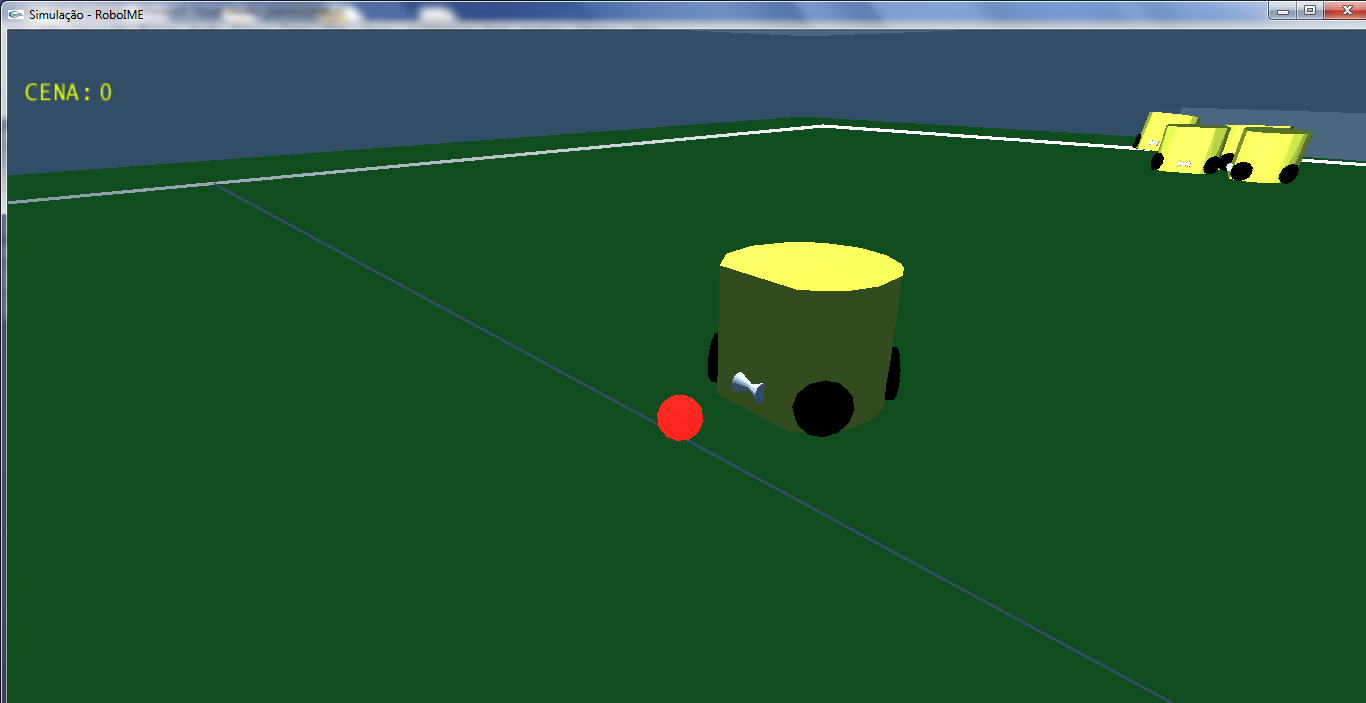
\includegraphics[scale = 0.36]{img/roboSim1.png}
	\caption{Simulated robot.}
	\label{roboSim}
\end{figure}

\subsection{Support Simulation Module}

	This module is part of F180 environment simulator. It simulates the physics of bodies presented in a match from the Small Size Robot League. Its also possible to make the control of robot actuators (motor, kicker and dribbler).

	The simulator was developed using the PhysX Engine, that enables high performance processing physics calculations in a GPU. Figure \ref{roboSim} shows the robot in the simulator. This module can provide long-terms predictions, in opposition to the Kalman Filter that provides a short-term prediction.

\subsection{Simulated World Module}
	This module is also part of the simulator designed to F180's environment. But this module replaces the
Real World, when it is not convenient to use it. Thus this module receives through UDP sockets the speeds that
the actuators of the robot must reach, the simulator has an internal controller to calculate the torque required
to be applied to the actuators to achieve the desired speed (like real robot).

\begin{figure}[thpb]
	\centering
%	\includegraphics[scale = 0.36]{simulacao1.png}
	\caption{Simulation environment of the F180.}
	\label{prototype}
\end{figure}

	The AI Module can configure the simulation environment of the Simulated World Module just sending an XML file,
via UDP Socket, containing information for the construction of bodies in the simulator. This module has two simulated
cameras which provide input to SSL-Vision, we use two OpenGL cameras and the images are sent through TCP sockets.

\subsection{Transmission Module}
	This module is responsible for delivering the speed to actuators and receiving status of the robot, such as real velocity
of each motor, kick sensor status and power supply status, via radio in Real World or via UDP socket in Simulation World. This
module is coded in CSharp language using the interface development Microsoft Visual Studio 2010 IDE.

\section{Path Planning}

Path planning algorithm is based on the theory of Artificial Potential Field \cite{CPA}, which has as its fundamental principle driving
the robot in an artificial force field generated by obstacles and the target. The potential (gradient) should be continuous.
The obstacles (other robots) and the target (certain objective local) generating fields of repulsion and attraction, respectively,
obtaining a movement by which avoids obstacles and possibly reach your goal.

%FAZER A PARTE DO A-ESTRELA

\section{Electronic Project}
RoboIME electronics consist of seven boards: (a) the Main board, responsible for communication between the other boards; (b) the Stamp board,
responsible  for the embedded computation; (c) the Kicker board, responsible for maintaining the high voltage to activate the kick shoot;
(d) four motor controller board which are responsible for robot's motion control. These boards are described in details in this section.

\subsection{Main Board}
The Main Board features a socket to plugin the boards: kick's sensor, dribble's motor, four wheel's motor, four encoders and the power supply.
There is a RFM12b SMD embedded which is a wireless transceiver operating in the 434 MHz band, set as up to 115.2 kbps, fully in agreement
with FCC and ETSI regulations.

The communication protocol used between the Stamp Board and the transceiver was Serial Peripheral Interface Bus (SPI), that  is a synchronous
serial data link standard that operates in full duplex mode.

\subsection{Stamp Board}
This board is responsible  for performing all the logic functions. It is like a brain of the electronic system. There is a embedded micro-controller STM32F407,
that has ARM Cortex M4 as main CPU, 1 MB Flash, 192 KB RAM memory, working in 168 MHz, that was programmed with C language using the  interface development
CoIDE and Eclipse IDE.
%vide http://www.st.com/st-web-ui/static/active/en/resource/sales_and_marketing/promotional_material/brochure/brstm32f4.pdf

\subsection{Kicker Board}
This board is responsible for controlling the kick strength. There are two kinds of kick,
the kick shoot and the high kick. Two capacitors of 2200 $\mu$F, 200 V are used store the
voltage in a boost circuit. The charge is discharged in a solenoid and depending on the PWM
signal the kick device is activated, it is possible to control the kick velocity.

%include image of high kick

\subsection{Motor Controller Board}
The idea of the RoboIME electronic is to modularize the electronic project. So, there
is controller module board for each wheel's motor. If one of them burns out, it is
possible to change quickly. Each board has two TC4427 (MOSFET driver) and two
IRF7319 (half H bridge). These ICs create a H-bridge, allowing velocity control in
both directions.

\section{Mechanical Project}

%%%%%%%%%%%%%%%%%%%%%%%%%%%COLOCAR OS DADOS REAIS DO NOSSO ROB              %%%%%%%%%%%%%%%%%%%%%%%%
In compliance with the SSL rules, the height of the robot is 148 mm, the maximum
percentage of ball coverage is 15\% and the maximum projection of the robot on the ground is 175 mm.
%%%%%%%%%%%%%%%%%%%%%%%%%%%COLOCAR OS DADOS REAIS DO NOSSO ROB              %%%%%%%%%%%%%%%%%%%%%%%%

With the aid of CAD software (Computer Aided Design) and CAM (Computer Aided
Manufacturing) a new robot has been developed. Figure \ref{mec} shows mechanical
3D view and real view of the robot. Shelf had been used allows omnidirectional
movement and has a greater torque that couples the fourth motors (one for each
wheel) for the movement.

\begin{figure}[thpb]
	\centering
	\subfigure[]{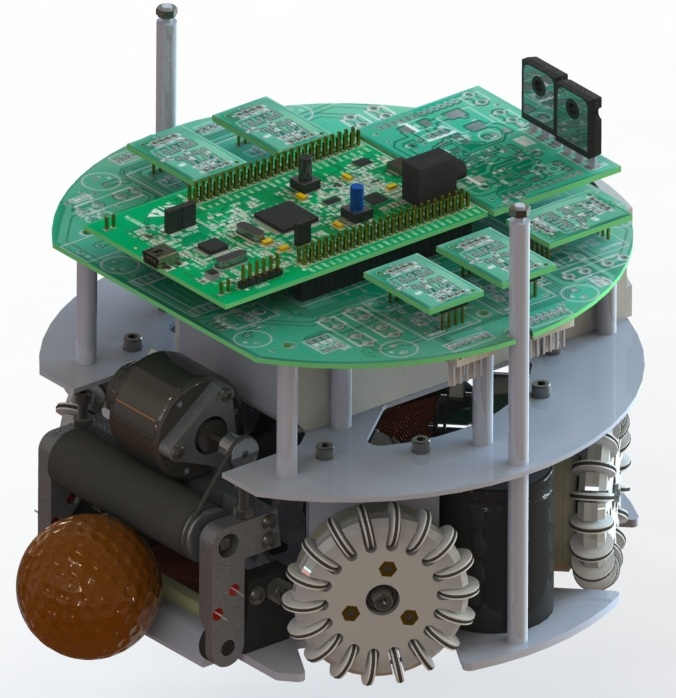
\includegraphics[width = 0.425 \textwidth]{img/cad.jpg}}
	\subfigure[]{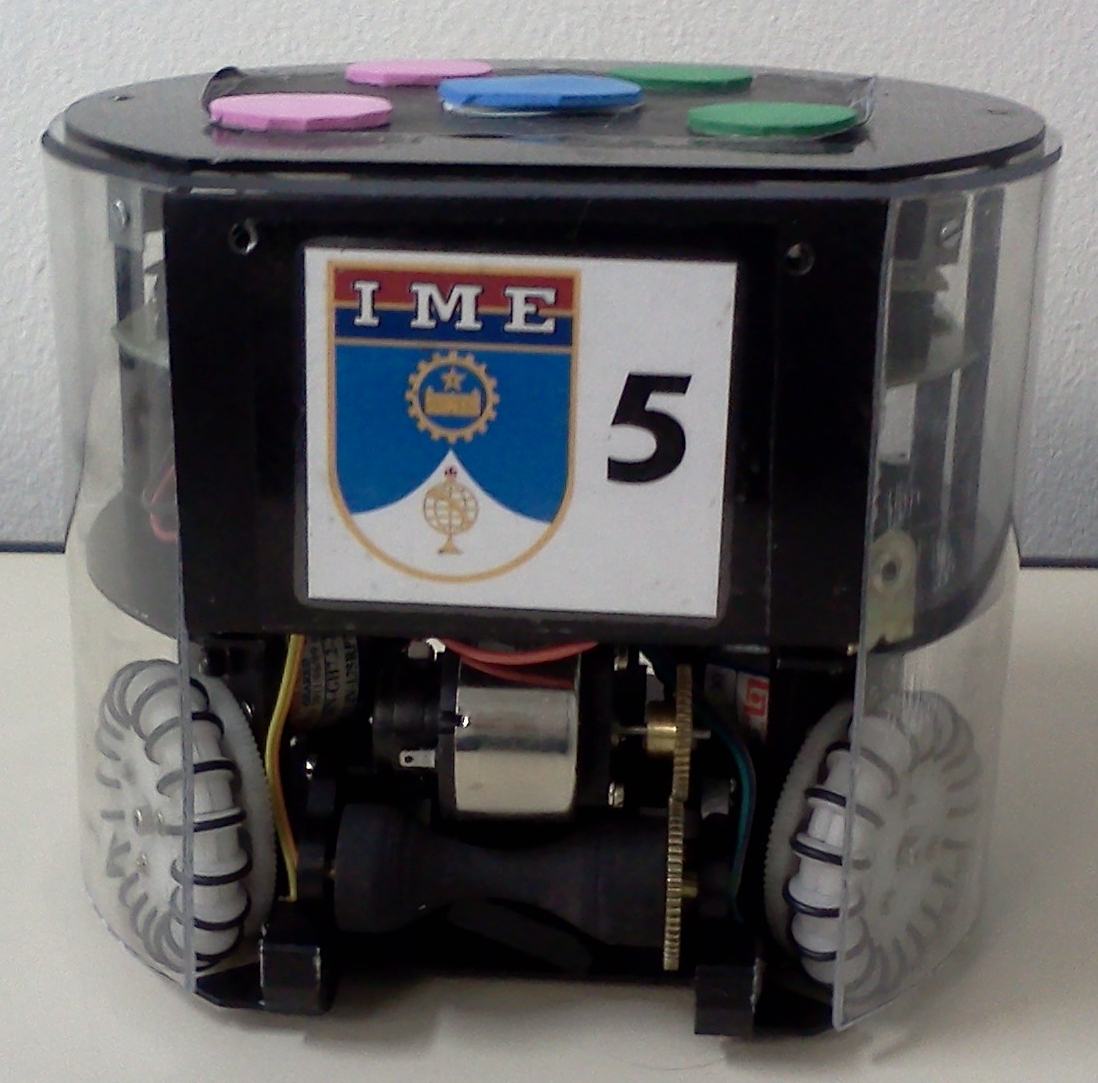
\includegraphics[width = 0.4 \textwidth]{img/robo.jpeg}}
	\caption{(a) Mechanical 3D model view. (b) Robot view.}
	\label{mec}
\end{figure}

The changes in the original design of the model provides a lower weight to
the robot, such as: changing the steel shaft by a shaft of high-strength
aluminium wheels and replacement of aluminium by plastic wheels Polytec
1000. This new design also enables more devices to be shipped. It presents
a diameter of 175 mm and an upper base with holes which give versatility
to the coupling. The fairing of the robot was made from polyvinyl plates.

\section{Final Comments}
The development of the Robocup 2014 mechanical project was concluded last year,
based on the one we created for Brazilian Robotics Competition 2012. The six
robots have already been manufactured, with only a few parts still needing rework.

Some electronic prototypes were made, yet stabilizing efforts are still ongoing.
Problems with kicker board due to hight welding temperature were observed. The solution
was to use a welding temperature below 260$^o$C.

The five modules of the AI system have already been implemented but they still
need to be brought to perfection.

Research in machine learning was started last year to predict enemy behaviour,
but an implementation is not planned for Robocup 2014.

To the June competition, following goals are being sought:
rework the remaining parts on the mechanical project such as making improvements on the coiling of the solenoid coil;
stabilize the electronic project, including robot feedback and
conclude the implementation of planning algorithms to be used in support decision making.

\section*{Acknowledgements}
This research was partially supported by Fundação Carlos Chagas Filho de Amparo a Pesquisa do Estado do Rio de Janeiro -FAPERJ(grant E-26/111.362/2012);
Fundação Ricardo Franco (FRF) and Fabrica de Material de Comunicação e Eletrônica (FMCE/IMBEL). The team also acknowledges the assistance of Mr. Carlos
Beckhauser from FMCE. Special thanks to Diego F. de Almeida, Luis R. L. Rodrigues, Stefano H. Rodrigues, Thiago A. N. do Amaral and Vitor L. H. Ferreira,
old team members that made this project possible.

\begin{thebibliography}{7}
%%%%%%%%%%%%%%%%%%%%%%

\bibitem{alexandre}
Alexandre Tadeu Rossini da Silva:
Comportamento social cooperativo na realização de tarefas em
ambientes dinâmicos e competitivos.
Instituto Militar de Engenharia, Rio de Janeiro (2006)

\bibitem{tdp}
Madeira, B.~E., de~Almeida, D.~F., de~C.~Maia~Jr., E., Rodrigues, L. R.~L.,
  Rosa, P. F.~F., Rodrigues, S.~H., and do~Amaral, T. A.~N.:
RoboIME: Team Description Paper for RoboCup 2012.

\bibitem{STP}
B. Browning and J. Bruce and M. Bowling and M. Veloso:
STP: Skills, tactics and plays for multi-robot control in adversarial environments
Carnegie Mellon University, Pittsburgh, PA (2004)

\bibitem{CPA}
Khatib, O.:
Real-Time Obstacle Avoidance for Manipulators and Mobile Robots.
In International Journal of Robotics Research, vol. 5, no. 1, p. 90-98 (1986)

\bibitem{marco}
Marco Antonio Firmino de Sousa:
Uma Plataforma para Cooperação Autónoma de Múltiplos Robôs
Instituto Militar de Engenharia, Rio de Janeiro (2008)

\bibitem{minimax} Russell, Stuart J.; Norvig, Peter:
Artificial Intelligence: A Modern Approach (2nd ed.)
Upper Saddle River, New Jersey: Prentice Hall, pp. 163-171 (2003)

\bibitem{zickler}
Stefan Zickler:
Physics-Based Robot Motion Planning in Dynamic Multi-Body Environments
Carnegie Mellon University, Pittsburgh, PA (2010)

\bibitem {ekf}
Welch, G. and Bishop, G.:
An introduction to the Kalman filter. Technical Report TR 95-041, Department of
Computer Science, University of North Carolina (2001)


%\bibitem{simCamera}
%Stefan Zickler, Olivier Michel:
%SSL-vision Webots integration
%http://youtu.be/sRAVELC8jKM, 26/02/2012


\end{thebibliography}

\end{document}
